%% GENERATED by make_eventzoom.py -- do not edit by hand.
\documentclass[border=4pt]{standalone}
\usepackage[T1]{fontenc}
\usepackage{helvet}
\renewcommand\familydefault{\sfdefault}
\usepackage{tikz}
\usepackage{pgfplots}
\pgfplotsset{compat=1.18}

\definecolor{ohqblue}{HTML}{1F5C8B}
\definecolor{ohqteal}{HTML}{2A9D8F}
\definecolor{ohqrust}{HTML}{E76F51}
\definecolor{ohqgrey}{HTML}{6B7280}

\begin{document}
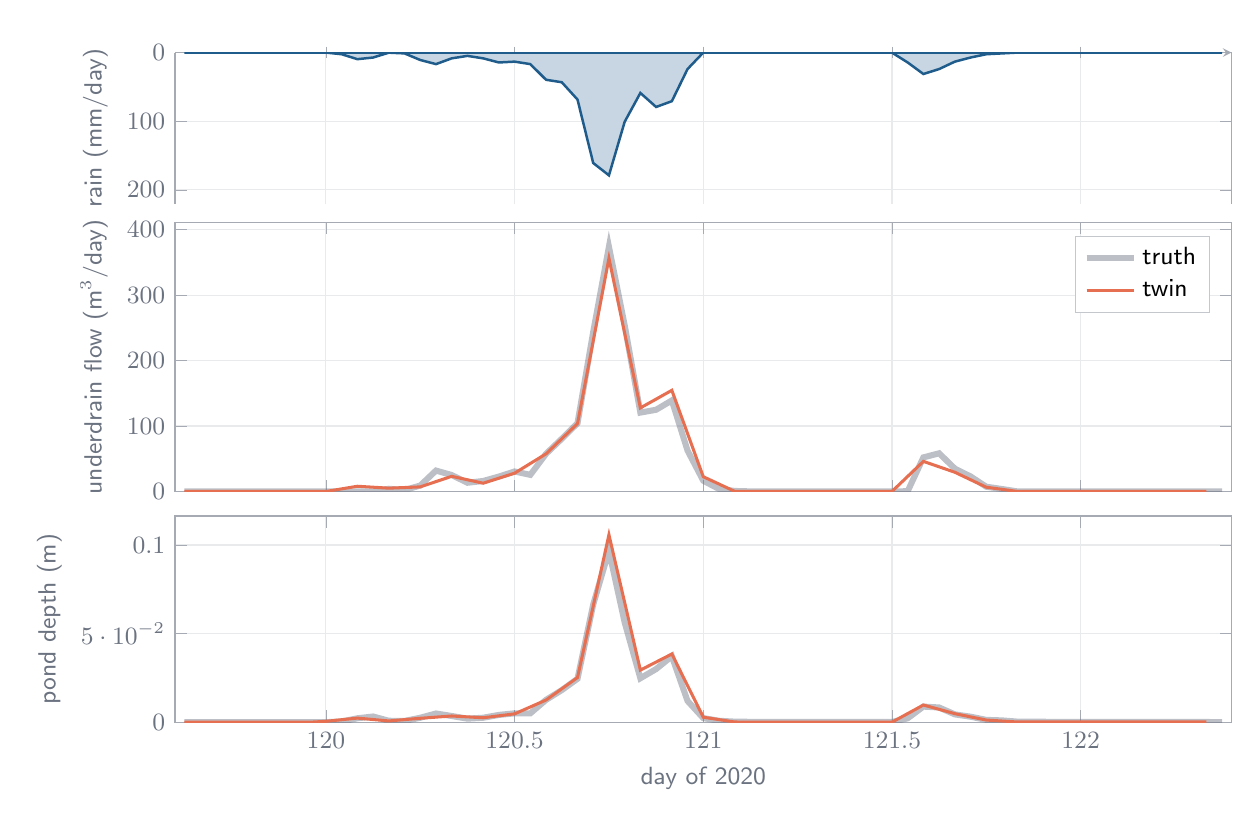
\begin{tikzpicture}[font=\sffamily]
\pgfplotsset{every axis/.append style={
  width=15cm, xmin=119.600, xmax=122.400,
  label style={font=\small, text=ohqgrey},
  tick label style={font=\small, text=ohqgrey},
  axis line style={ohqgrey!60}, tick style={ohqgrey!60},
  grid=major, major grid style={ohqgrey!15},
  xtick={120.0,120.5,121.0,121.5,122.0},
}}

\begin{axis}[name=rain, height=3.5cm,
  ylabel={rain (mm/day)}, ymin=0, ymax=220, ytick={0,100,200},
  xticklabels={}, y dir=reverse, axis x line=top, xticklabel pos=top,
  xticklabels={}]
\addplot[ohqblue, line width=0.9pt, fill=ohqblue!25] coordinates {(119.6250,0.0000) (119.6667,0.0000) (119.7083,0.0000) (119.7500,0.0000) (119.7917,0.0000) (119.8333,0.0000) (119.8750,0.0000) (119.9167,0.0000) (119.9583,0.0000) (120.0000,0.0000) (120.0417,2.4000) (120.0833,9.6000) (120.1250,7.2000) (120.1667,0.1369) (120.2083,1.2000) (120.2500,10.8000) (120.2917,16.8000) (120.3333,8.4000) (120.3750,4.8000) (120.4167,8.4000) (120.4583,14.4000) (120.5000,13.2000) (120.5417,16.8000) (120.5833,39.6000) (120.6250,43.2000) (120.6667,68.4000) (120.7083,160.8000) (120.7500,178.8000) (120.7917,100.8000) (120.8333,58.8000) (120.8750,79.2000) (120.9167,70.8000) (120.9583,24.0000) (121.0000,0.0000) (121.0417,0.0000) (121.0833,0.0000) (121.1250,0.0000) (121.1667,0.0000) (121.2083,0.0000) (121.2500,0.0000) (121.2917,0.0000) (121.3333,0.0000) (121.3750,0.0000) (121.4167,0.0000) (121.4583,0.0000) (121.5000,0.0000) (121.5417,14.4000) (121.5833,31.2000) (121.6250,24.0000) (121.6667,13.2000) (121.7083,7.2000) (121.7500,2.4000) (121.7917,1.2000) (121.8333,0.0000) (121.8750,0.0000) (121.9167,0.0000) (121.9583,0.0000) (122.0000,0.0000) (122.0417,0.0000) (122.0833,0.0000) (122.1250,0.0000) (122.1667,0.0000) (122.2083,0.0000) (122.2500,0.0000) (122.2917,0.0000) (122.3333,0.0000) (122.3750,0.0000)} \closedcycle;
\end{axis}

\begin{axis}[name=flow, at={(rain.below south west)}, anchor=north west,
  yshift=-2pt, height=5.0cm,
  ylabel={underdrain flow (m$^3$/day)}, ymin=0, xticklabels={},
  legend style={font=\small, draw=ohqgrey!40, at={(0.98,0.95)},
                anchor=north east, fill=white},
  legend cell align=left]
\addplot[ohqgrey, line width=2.2pt, opacity=0.45] coordinates {(119.6250,0.0000) (119.6667,0.0000) (119.7083,0.0000) (119.7500,0.0000) (119.7917,0.0000) (119.8333,0.0000) (119.8750,0.0000) (119.9167,0.0000) (119.9583,0.0000) (120.0000,0.0000) (120.0417,0.0000) (120.0833,0.0000) (120.1250,0.0000) (120.1667,4.1128) (120.2083,2.1705) (120.2500,9.0968) (120.2917,31.9125) (120.3333,25.1217) (120.3750,13.3289) (120.4167,16.0036) (120.4583,22.7619) (120.5000,30.5129) (120.5417,25.3880) (120.5833,57.5244) (120.6250,80.4773) (120.6667,104.2470) (120.7083,243.6460) (120.7500,373.7770) (120.7917,254.0680) (120.8333,120.5150) (120.8750,124.8090) (120.9167,139.0860) (120.9583,62.5047) (121.0000,16.4370) (121.0417,3.8994) (121.0833,0.7780) (121.1250,0.1203) (121.1667,0.0000) (121.2083,0.0000) (121.2500,0.0000) (121.2917,0.0000) (121.3333,0.0000) (121.3750,0.0000) (121.4167,0.0000) (121.4583,0.0000) (121.5000,0.0000) (121.5417,0.3887) (121.5833,52.0279) (121.6250,58.3082) (121.6667,34.9093) (121.7083,22.9921) (121.7500,7.2373) (121.7917,3.7525) (121.8333,0.0000) (121.8750,0.0000) (121.9167,0.0000) (121.9583,0.0000) (122.0000,0.0000) (122.0417,0.0000) (122.0833,0.0000) (122.1250,0.0000) (122.1667,0.0000) (122.2083,0.0000) (122.2500,0.0000) (122.2917,0.0000) (122.3333,0.0000) (122.3750,0.0000)};
\addlegendentry{truth}
\addplot[ohqrust, line width=1.1pt] coordinates {(119.6250,0.0000) (119.7083,0.0000) (119.7917,0.0000) (119.8750,0.0000) (119.9583,0.0000) (120.0000,0.0000) (120.0833,7.9734) (120.1667,5.0520) (120.2500,6.9948) (120.3333,23.1512) (120.4167,12.6143) (120.5000,27.9617) (120.5833,57.4705) (120.6667,103.7230) (120.7500,356.2260) (120.8333,127.6290) (120.9167,154.5280) (121.0000,22.5564) (121.0833,0.1908) (121.1667,0.1545) (121.2500,0.1181) (121.3333,0.0818) (121.4167,0.0454) (121.5000,0.0091) (121.5833,45.9814) (121.6667,29.3537) (121.7500,6.5205) (121.8333,0.0000) (121.9167,0.0000) (122.0000,0.0000) (122.0833,0.0000) (122.1667,0.0000) (122.2500,0.0000) (122.3333,0.0000)};
\addlegendentry{twin}
\end{axis}

\begin{axis}[name=depth, at={(flow.below south west)}, anchor=north west,
  yshift=-2pt, height=4.2cm,
  xlabel={day of 2020}, ylabel={pond depth (m)}, ymin=0]
\addplot[ohqgrey, line width=2.2pt, opacity=0.45] coordinates {(119.6250,0.0000) (119.6667,0.0000) (119.7083,0.0000) (119.7500,0.0000) (119.7917,0.0000) (119.8333,0.0000) (119.8750,0.0000) (119.9167,0.0000) (119.9583,0.0000) (120.0000,0.0000) (120.0417,0.0004) (120.0833,0.0022) (120.1250,0.0032) (120.1667,0.0008) (120.2083,0.0007) (120.2500,0.0025) (120.2917,0.0049) (120.3333,0.0035) (120.3750,0.0020) (120.4167,0.0025) (120.4583,0.0041) (120.5000,0.0050) (120.5417,0.0050) (120.5833,0.0126) (120.6250,0.0181) (120.6667,0.0245) (120.7083,0.0664) (120.7500,0.0968) (120.7917,0.0563) (120.8333,0.0248) (120.8750,0.0300) (120.9167,0.0372) (120.9583,0.0120) (121.0000,0.0023) (121.0417,0.0008) (121.0833,0.0003) (121.1250,0.0002) (121.1667,0.0002) (121.2083,0.0001) (121.2500,0.0001) (121.2917,0.0001) (121.3333,0.0001) (121.3750,0.0001) (121.4167,0.0001) (121.4583,0.0001) (121.5000,0.0001) (121.5417,0.0022) (121.5833,0.0088) (121.6250,0.0083) (121.6667,0.0044) (121.7083,0.0031) (121.7500,0.0013) (121.7917,0.0010) (121.8333,0.0003) (121.8750,0.0003) (121.9167,0.0002) (121.9583,0.0002) (122.0000,0.0001) (122.0417,0.0001) (122.0833,0.0001) (122.1250,0.0001) (122.1667,0.0001) (122.2083,0.0001) (122.2500,0.0001) (122.2917,0.0001) (122.3333,0.0001) (122.3750,0.0000)};
\addplot[ohqrust, line width=1.1pt] coordinates {(119.6250,0.0000) (119.7083,0.0000) (119.7917,0.0000) (119.8750,0.0000) (119.9583,0.0000) (120.0000,0.0005) (120.0833,0.0023) (120.1667,0.0007) (120.2500,0.0022) (120.3333,0.0035) (120.4167,0.0025) (120.5000,0.0047) (120.5833,0.0125) (120.6667,0.0252) (120.7500,0.1058) (120.8333,0.0294) (120.9167,0.0385) (121.0000,0.0028) (121.0833,0.0001) (121.1667,0.0000) (121.2500,0.0000) (121.3333,0.0000) (121.4167,0.0000) (121.5000,0.0000) (121.5833,0.0097) (121.6667,0.0048) (121.7500,0.0012) (121.8333,0.0001) (121.9167,0.0001) (122.0000,0.0001) (122.0833,0.0001) (122.1667,0.0001) (122.2500,0.0001) (122.3333,0.0001)};
\end{axis}

\end{tikzpicture}
\end{document}
